\section{The Artificial Neural Networks}

The human brain is composed of a big set of specialized cells (\textit{neurons}) connected among them, which memorize and process information, thus controlling the body activities they belong to as depicted in \figref{fig:brain}. The human brain is probably the most remarkable result of evolution for its ability to elaborate information. 
The Artificial Neural Networks are mathematical models that represent the interconnection between elements defined "Artificial Neurons", mathematical constructs that somehow imitate the properties of biological neurons, going to reproduce the functioning of the human nervous system.

\subsection{The Human Nervous System} 

\begin{figure}[t]
\centering
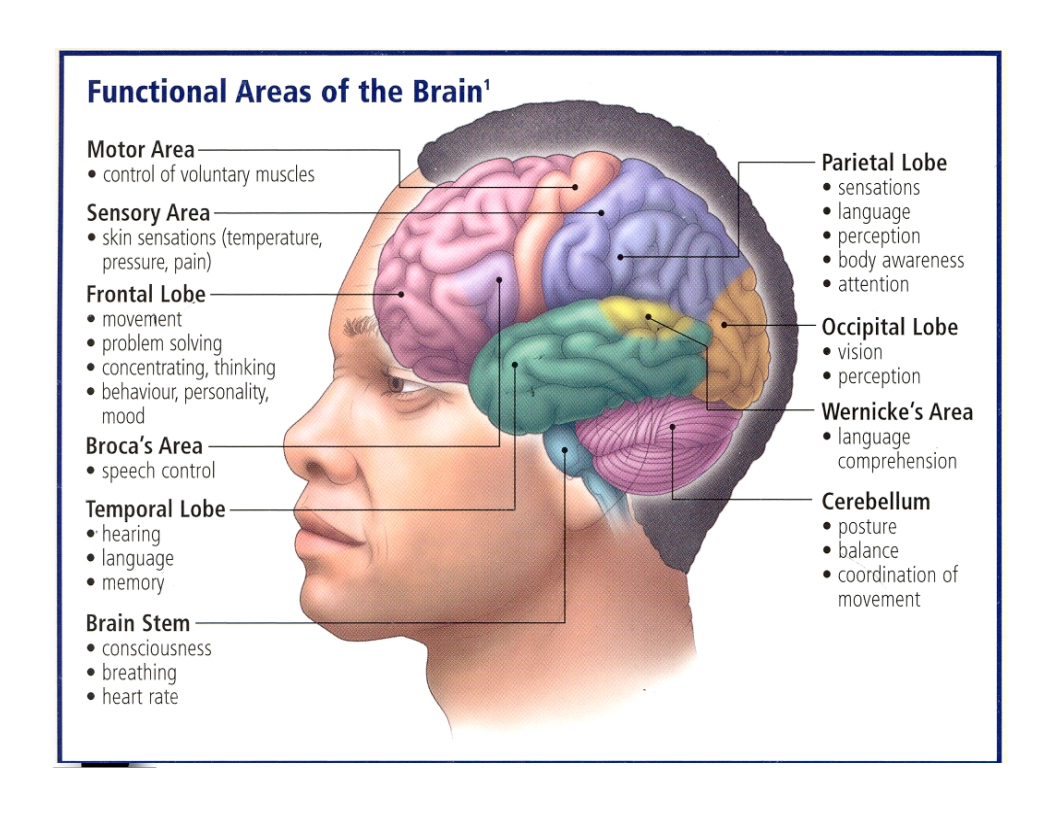
\includegraphics[width=0.95\linewidth]{img/Brain}
\caption[Human Brain]{The human brain.}
\label{fig:brain}
\end{figure}

The biological neuron is composed of three main parts: the cell body is named \textit{Soma}, which is the calculation unit, the \textit{Axon}, that acts as a transmission line output and the \textit{Dendrites}, that are receptive areas and that receive input signals from other axons via the syurons. The cell body performs a weighted sum (integration) of the input signals. If the result exceeds a certain threshold value then the neuron is active and the \textit{action potential}  is produced and transmitted through the Axon. If the result does not exceed the threshold valuem, the napses. 
Synapses are the functional units of the elementary structure that manages the iterations between neneuron remains in a state of rest. 
The Biological neurons (\figref{fig:neuron}) are electro-chemical devices, operating at low rates (approximately in the order of milliseconds), while digital circuits operate at very high rates (nanoseconds).

\begin{figure}[t]
\centering
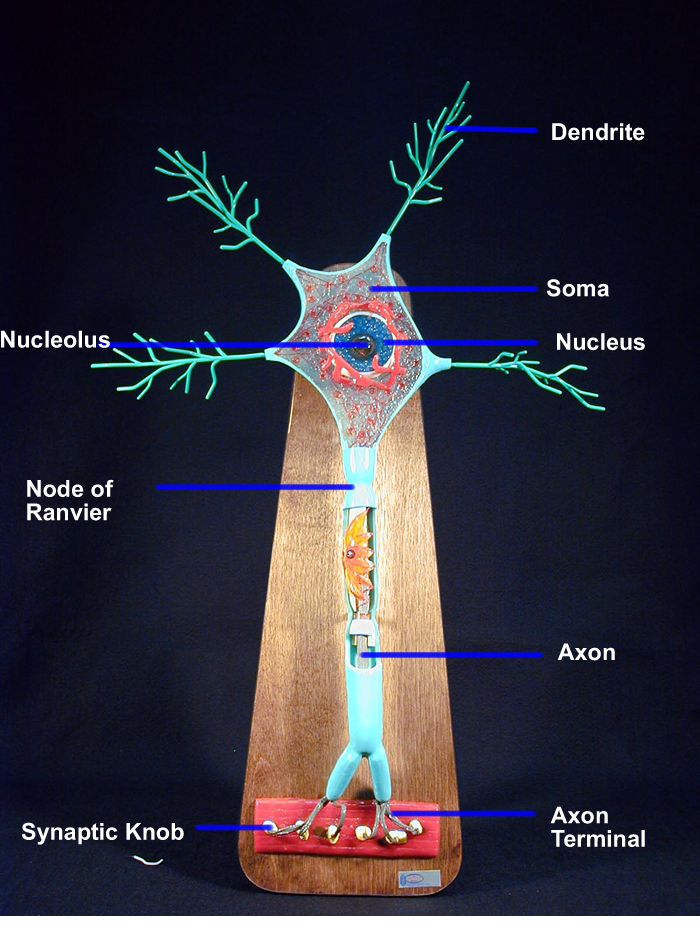
\includegraphics[width=0.5\linewidth]{img/neuron_model}
\caption[Neuron Model]{The neuron model.}
\label{fig:neuron}
\end{figure}

The \textit{neuron} properties can be described in:
\begin{itemize}
\item \textit{local simplicity}: the neuron receives stimuli (excitation or inhibition) from dendrites and produces an impulse to the axon which is proportional to the weighted sum of the inputs;
\item \textit{global complexity}: the human brain possess 
$\mathcal{O}(10^{10})$ 
neurons, with more than 10k connections each;
\item \textit{learning}: even though the network topology is relatively fixed, the strength of connections (synaptic weights) can change when the network is exposed to external stimuli;
\item \textit{distributed control}: no centralized control, each neuron reacts only to its own stimuli;
\item \textit{tolerance to failures}: performance slowly decrease with the increase of failures.
\end{itemize}

The biological Neural Networks are able to solve very complex tasks in few time instants (like memorization, recognition, association, and so on.)

\subsection{Fundamentals of the Artificial Neural Networks} 

An artificial neural network (ANN), is a mathematical/informatical model calculation based on biological neural networks.
This model is constituted by a group of interconnections of information consisting of artificial neurons and processes using a connectionist approach to computation. In most cases, an artificial neural network is an adaptive system that changes its structure, which is based on external or internal information that flows through the network during the learning phase. 
In practical terms neural networks are non-linear structures of statistical data organized as modeling tools.
They can be used to simulate the complex relationships between inputs and outputs that other analytic functions fail to represent.
An artificial neural network receives external signals on a layer of nodes (processing unit) input, each of which is connected with a number of internal nodes, organized in several levels. Each node processes the received signals performing a very simple task  and transmits the result to subsequent nodes. 

\begin{figure}[h]
	\centering
	\resizebox{1.05\textwidth}{!}{
	\begin{tikzpicture}[
init/.style={
  draw,
  circle,
  inner sep=2pt,
  font=\Huge,
  join = by -latex
},
squa/.style={
  draw,
  inner sep=2pt,
  font=\Large,
  join = by -latex
},
start chain=2,node distance=13mm
]
\node[on chain=2] 
  (x2) {$x_2$};
\node[on chain=2,join=by o-latex] 
  {$w_2$};
\node[on chain=2,init] (sigma) 
  {$\displaystyle\Sigma$};
\node[on chain=2,squa,label=above:{\parbox{2cm}{\centering Activate \\ function}}]   
  {$f$};
\node[on chain=2,label=above:Output,join=by -latex] 
  {$y$};
\begin{scope}[start chain=1]
\node[on chain=1] at (0,1.5cm) 
  (x1) {$x_1$};
\node[on chain=1,join=by o-latex] 
  (w1) {$w_1$};
\end{scope}
\begin{scope}[start chain=3]
\node[on chain=3] at (0,-1.5cm) 
  (x3) {$x_3$};
\node[on chain=3,label=below:Weights,join=by o-latex] 
  (w3) {$w_3$};
\end{scope}
\node[label=above:\parbox{2cm}{\centering Bias \\ $b$}] at (sigma|-w1) (b) {};

\draw[-latex] (w1) -- (sigma);
\draw[-latex] (w3) -- (sigma);
\draw[o-latex] (b) -- (sigma);

\draw[decorate,decoration={brace,mirror}] (x1.north west) -- node[left=10pt] {Inputs} (x3.south west);
\end{tikzpicture}
	}
	\caption[Artificial Neuron Model]{The artificial neuron model.}
	\label{fig:artificial_neuron}
	\end{figure}


The artificial neuron is an information-processing unit that is fundamental to the operation of a neural network. The model of a neuron is composed of three basic elements, as shown in (\figref{fig:artificial_neuron}) 

\begin{itemize}
\item a \textit{set of synapses}, or connecting links, each of which is characterized by a weight or strength of its own, $w_{km}$; The neural model also includes an externally applied \textit{bias}, denoted by $b_k$.
\item an \textit{adder} for summing the input signals, weighted by the respective synaptic strengths of the neuron; the operations described here constitute a linear combiner;
\item an \textit{activation function} for limiting the amplitude of the output of a neuron. Typically, the normalized amplitude range of the output of a neuron is written as the closed unit interval [0,1], or, alternatively, [-1,1].
\end{itemize}
%The mathematical description of neuron activity can be defined as:
%\begin{eqnarray}
%{ u }_{ k }=\sum _{ j=1 }^{ m }{ { w }_{ kj } } { x }_{ j }\\ 
%{ y }_{ k }=\varphi \left( { u }_{ k }+b_{ k } \right)
%\end{eqnarray}
%where: ${ x }_{ 1 },{ x }_{ 2 },\cdots ,{ x }_{ m }$ are the input signals, ${ w }_{ k1 },{ w }_{ k2 },\cdots ,{ w }_{ km }$ are the respective synaptic weights of neuron $k$, $u_k$ is the linear combiner output due to the input signals, $b_k$ is the bias, $\varphi(\cdot)$ is the activation function and $y_k$ is the output signal of the neuron.
The most typical non-linear function $\varphi(x)$ employed as activation functions are:
\begin{itemize}
\item the \textit{sigmoid function}: it is defined as a strictly increasing function that exhibits a graceful balance between linear and nonlinear behavior; an example of the sigmoid function is the \textit{logistic function} defined by:

\begin{equation}
\varphi \left( v \right) =\frac { 1 }{ 1+exp\left( -av \right)  } 
\end{equation}


\item the \textit{ hyperbolic tangent } ($tanh$): it is simply a scaled and shifted version of the sigmoid function, defined as:

\begin{equation}
\varphi(x) = \frac{1-e^{-2x}}{1+e^{-2x}}
\end{equation}


\begin{figure}[h]
	\centering
	\resizebox{0.4\textwidth}{!}{
	\begin{tikzpicture}
\begin{axis}[
    xmin=-2.5, xmax=2.5,
    ymin=-1.5, ymax=1.5,
    axis lines=center,
    axis on top=true,
    domain=-2.5:2.5,
    ylabel=$y$,
    xlabel=$x$,
    ]

    \addplot [mark=none] {tanh(\x)};
    \node [right] at (axis cs: 1,0.7) {$y = \tanh x$};

    %% Add the asymptotes
    \draw [dotted, thick] (axis cs:-2.5,-1)-- (axis cs:0,-1);
    \draw [dotted, thick] (axis cs:+2.5,+1)-- (axis cs:0,+1);
\end{axis}
\end{tikzpicture}}
\caption[The $tanh$]{The $tanh$ non-linear function.}
\end{figure}


\item the \textit{ Rectifier Linear Unit} ($ReLU$):
\begin{equation}
\varphi(x) = \text{max}(0,x)
\end{equation}
%\begin{figure}[h!]
%\centering
%	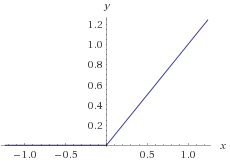
\includegraphics[width=0.4\textwidth]{img/relu}
%	\caption{The $ReLU$ non-linear function.}
%\end{figure}
\begin{figure}[h!]
	\centering
	\resizebox{0.4\textwidth}{!}{
	\begin{tikzpicture}[]
\begin{axis}[
	domain=-3:5,
	axis lines=center,
	axis on top=true,
	ylabel=$y$,
	xlabel=$x$,
	]
	\addplot+[mark=none,black,domain=-3:0] {0};
	\addplot+[mark=none,black,domain=0:4] {x};
	\node [right] at (axis cs: 1,0.7) {$y = x$};
\end{axis}
\end{tikzpicture}}
	\caption[The $ReLU$]{The $ReLU$ non-linear function.}
\end{figure}

\item the $softmax$: it is used on the last layer of a classifier setup: the outputs of the softmax layer represent the probabilities that a sample belongs to the different classes. Indeed, the sum of all the output is equal to $1$.
\begin{equation}
\varphi(x_k) = \frac{e^{x_k}}{\sum_{j=1}^{N}e^{x_j}} \text{ for }  k=1,\dots,K
\end{equation}
\end{itemize}

% ****************************************************+
\vspace{0.5cm}
The link input-output, which is the transfer function of the network, is not programmed but is simply obtained by a learning process based on empirical data. At the beginning of the training procedure, the weights ${ w }_{ km }$ are randomly initialized, and they are adjusted as learning proceeds. 
There are three major learning paradigms, each corresponding to a particular abstract learning task.
They are supervised learning, unsupervised learning, and reinforcement learning. Usually a type of
network architecture may be used in each of these tasks:
\begin{itemize}
	\item \textit{the Supervised Learning:} is used if is available a set of data for the training comprising typical examples of the inputs and their corresponding outputs: in this way the network can learn to infer the relation that binds them. Subsequently, the network is trained by means of an appropriate algorithm (typically, the backpropagation which is precisely a supervised learning algorithm), which uses such data for the purpose of modifying the weights and other parameters of the network to minimize the estimation error for the whole training. If the training is successful, the network learns to recognize the unknown relationship that binds the input variables to the output, and is therefore able to make predictions even where the output is not known a priori; in other words, the final objective supervised learning is the prediction of the output value for each valid value input, relying only on a limited number of examples of correspondence. To do this, the network must be finally provided with an adequate generalization ability, with reference to cases unknown to it. This will solve the problems of regression or classification;
	
	\item \textit{The Reinforcement Learning:} The algorithms for reinforcement learning ultimately trying to determine a policy to maximize the incentives	received by the agent accumulated in the course of its exploration of the problem. The reinforcement learning differs from the supervised because it has never seen pairs of input-output examples known, nor shall correct explicit suboptimal actions.
	In addition, the algorithm is focused on the online use, which implies a balance between exploitation and exploration of unknown situations of current knowledge;
	
	\item \textit{The non-Supervised Learning:} is based on training algorithms that modify the network weights only	by reference to a set of data that includes just the input variables. These algorithms attempt to group the input data and therefore to identify the appropriate cluster representative of the data, typically by making use of topological methods or probabilistic. The unsupervised learning is also used to develop techniques for data compression.
	
\end{itemize}

% *********************************************************+
\section{Deep Neural Network Architectures for Analysis of Sound Events}

The manner in which the neurons of a neural network are structured is intimately linked with the task they are designed for. Hereafter, a brief description of the neural network architectures employed in this work for the analysis of sound events is provided.


\subsection{Multi Layer Perceptron (MLP)}

%\begin{figure}[h]
%	\centering
%	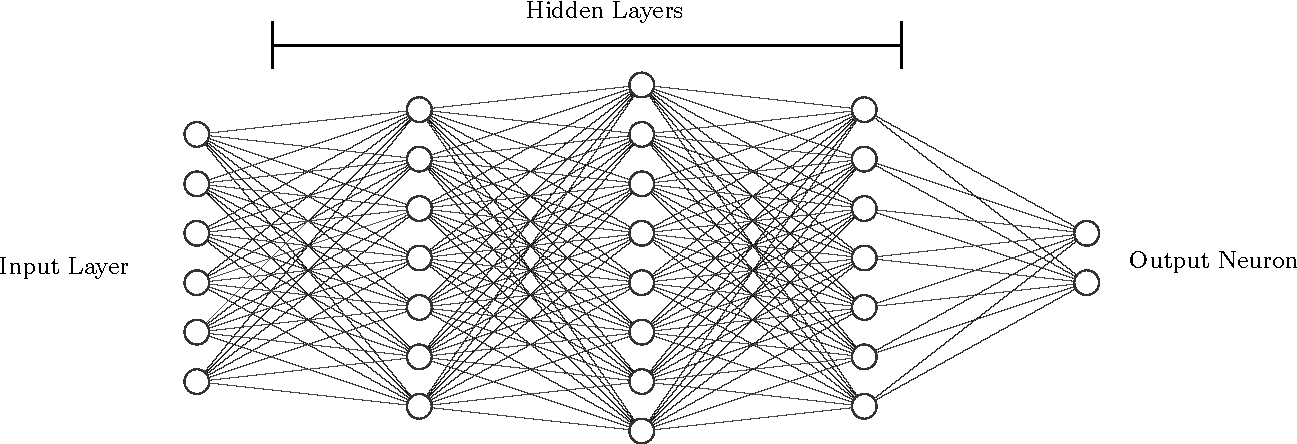
\includegraphics[width=0.9\textwidth]{img/mlp}
%	\caption{The MLP Neural Network.}
%	\label{fig:ANN}
%\end{figure}

\begin{figure}[h]
	\centering
	\resizebox{0.75\textwidth}{!}{
	\begin{tikzpicture}[
plain/.style={
  draw=none,
  fill=none,
  },
net/.style={
  matrix of nodes,
  nodes={
    draw,
    circle,
    inner sep=10pt
    },
  nodes in empty cells,
  column sep=2cm,
  row sep=-9pt
  },
>=latex
]
\matrix[net] (mat)
{
|[plain]| \parbox{1.3cm}{\centering Input\\layer} & |[plain]| \parbox{1.3cm}{\centering Hidden\\layer} & |[plain]| \parbox{1.3cm}{\centering Output\\layer} \\
& |[plain]| \\
|[plain]| & \\
& |[plain]| \\
  |[plain]| & |[plain]| \\
& & \\
  |[plain]| & |[plain]| \\
& |[plain]| \\
  |[plain]| & \\
& |[plain]| \\    };
\foreach \ai [count=\mi ]in {2,4,...,10}
  \draw[<-] (mat-\ai-1) -- node[above] {Input \mi} +(-2cm,0);
\foreach \ai in {2,4,...,10}
{\foreach \aii in {3,6,9}
  \draw[->] (mat-\ai-1) -- (mat-\aii-2);
}
\foreach \ai in {3,6,9}
  \draw[->] (mat-\ai-2) -- (mat-6-3);
\draw[->] (mat-6-3) -- node[above] {Ouput} +(2cm,0);
\end{tikzpicture}}
	\caption[MLP]{The MLP Neural Network.}
	\label{fig:ANN}
\end{figure}

The Multi Layer Perceptron (MLP) or Multilayer Feedforward Network is characterized by the presence of one or more hidden layers, whose computation nodes are correspondingly called \textit{hidden neurons}.
The MLP is one of the first ``deep'' architectures being introduced in 1986 \cite{Rumelhart86-LRB}. Artificial Neural Networks are often referred as deep when they have more than 1 or 2 hidden layers.
Indeed, it is well known that an  MLP with one or more hidden layers and a sufficient number of non-linear units (neurons) can  approximate any continuous  function  on  a  compact  input  domain  with arbitrary precision.
Each node applies an activation function over the weighted sum of its inputs. 
The units are arranged in layers, with feed forward connections from one layer to the next. 
The behaviour of this architecture  is  parametrized  by  the connection weights, which are adapted during the supervised network training.
In the forward pass, input examples are fed to the input layer, and the resulting output is propagated via the hidden layers towards the output layer. At the backward pass, the error signal originating at the output neurons is sent back through the layers and the network parameters (i.e., weights and biases) are tuned.

A single neuron can be formally described as:
\begin{equation}
g(\mathbf{u}[n])=\varphi \left(\sum _{ j=1 }^{ D }{w_j u_j[n] } + b\right),
\end{equation}
where $\mathbf{u}[n] \in \mathbb{R}^{D\times 1}$, the bias $b$ is an externally applied term and $\varphi(\cdot)$ is the non-linear activation function.
Thus, the mathematical description of a one-hidden-layer MLP is a function $\mathbf{f}:\mathbb{R}^D \rightarrow \mathbb{R}^{D'}$, where $D'$ is the size of the output vector, so:
\begin{equation}
\mathbf{f}(\mathbf{u}[n]) = 	\varphi \left( \mathbf{b}_2 + \mathbf{W}_2 \left( \varphi \left( \mathbf{b}_1 + \mathbf{W}_2 \cdot \mathbf{u}[n]\right) \right) \right),
\end{equation}
where $\mathbf{W}_i$ and $\mathbf{b}_{i}$ are the respective synaptic weights matrix and the bias vector of the $i$-th layer.

Regarding the computational complexity, considering additions and multiplications as separate operations, the total number of operations for each layer is given by 
\begin{equation}
\text{Cost}_{\text{MLP}} = \sum_{i=1}^P 2Q_{i-1}Q_i + \sum_{i=1}^{P} Q_i ,
\end{equation}
where $P$ is the number of layers, and $Q_i$ denotes the number of units of layer $i$. The first term, considers the number of operations for a linear unit, while the second term considers the operations required by the ReLU activation function (i.e., the maximum operation).

\subsection{Convolutional Neural Networks (CNN)}
\begin{figure}[h]
	 \centering
	 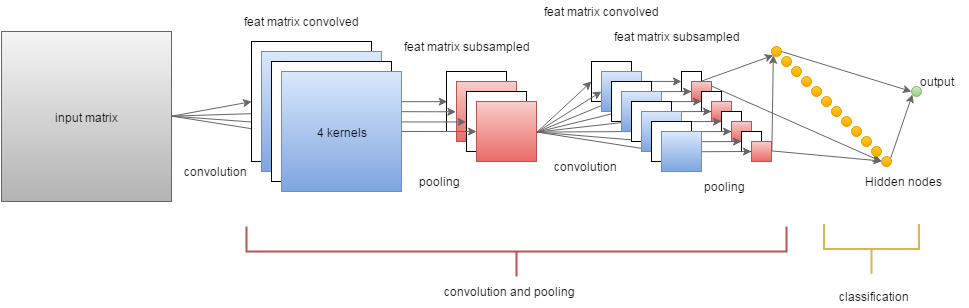
\includegraphics[width=\columnwidth]{img/CNN}
	 \caption[CNN]{The Convolutional Neural Network.}
	 \label{fig:cnn}
	\end{figure}


The birth of this kind of feed-forward neural network is related to image processing \cite{lawrence1997face}. Indeed, neural networks as MLPs take vectors as input, while this condition is not satisfied in the image case. The problem is tackled by means of convolutional layers, whose aim is to process restricted a area of a 2-D input, similarly to what happens in the animal visual cortex.
Convolution kernels process the input data matrix by dividing it in local \textit{receptive fields}, a region of the same size of the kernel, and sliding the local receptive field across the entire input.
Thus, the whole input matrix is processed by repeated application of a function across its sub-regions, obtaining so-called \textit{feature maps}. Practically, this is implemented by a convolution of the input data with a linear filter, adding a bias term and then applying a non-linear function.
The weights in each \textit{feature map} are \textit{shared}: all hidden neurons are aimed to detect exactly the same pattern just at different locations in the input image. The kernels are generally small compared to the input, allowing CNNs to process large inputs with few trainable parameters.

\begin{figure}[h]
	\centering
	\begin{subfigure}{0.5\columnwidth}
		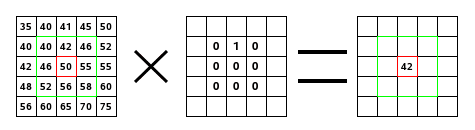
\includegraphics[width=\columnwidth]{img/convolution-calculate}
		\caption{}
	\end{subfigure}
	\begin{subfigure}{0.4\columnwidth}
		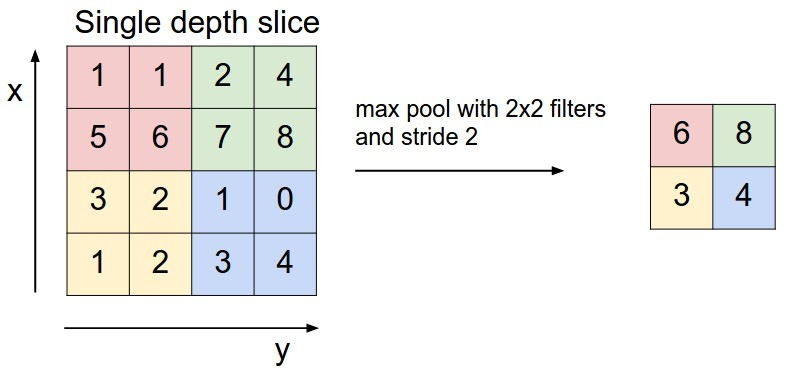
\includegraphics[width=\columnwidth]{img/maxpool.jpeg}
		\caption{}
	\end{subfigure}
	\caption[Convolution and Pooling]{Details of \textit{convolution} (a) and \textit{max-pooling} (b) operations.}
	\label{fig:convolution}	
\end{figure}


CNN is a feed-forward neural network \cite{726791} usually composed of three types of layers: convolutional layers, pooling layers and layers of neurons, as shown in \figref{fig:cnn}. Pooling layer just reduces the dimension of the matrix by a rule: a submatrix of the input is selected, and the output is the maximum value of this submatrix.
The pooling process introduces tolerance against shifts of the input patterns. Together with convolution layer it allows the CNN to detect if a particular event occurs, regardless its deformation or its position.
Finally, at the top of the network, a layer of neurons is applied. This layer does not differ from MLP, being composed by a set of activation and being fully connected with the previous layer. 

Denoting with $\mathbf{W}_{m} \in \mathbb{R}^{K_{1m}\times K_{2m}}$ the $m$-th kernel and with $\mathbf{b}_{m}  \in \mathbb{R}^{D_1\times D_2}$ the bias vector of a generic convolutional layer, the $m$-th feature map  $\mathbf{h}_{m} \in \mathbb{R}^{D_1\times D_2}$ is given by:
\begin{equation}
\label{eq:conv_op}
\mathbf{h}_{m}=\varphi	\left(\sum_{d=1}^{D_3} \mathbf{W}_{m} \ast \mathbf{u}_d + \mathbf{b}_{m} \right),
\end{equation}
where $\ast$ represent the convolution operation, and $\mathbf{u}_{d} \in \mathbb{R}^{D_1\times D_2} $ is a matrix of the three-dimensional input tensor $\mathbf{u} \in \mathbb{R}^{D_1\times D_2 \times D_3}$. The dimension of the $m$-th feature map $\mathbf{h}_{m}$ depends on the zero padding of the input tensor: here, padding is performed in order to preserve the dimension of the input, i.e., $\mathbf{h}_{m} \in \mathbb{R}^{D_1\times D_2}$. 

The computational complexity of the CNN is given by the sum of the computational complexity of the convolutional layers and of the fully connected layers. The complexity of convolutional layers can be obtained from \eqref{eq:conv_op} and from the number of operations of the max-pooling operator. Regarding the former, supposing square kernels, i.e., $K_{1m} = K_{1m} = K_m$, the number of operations required for calculating the feature map $\mathbf{h}_{m}$ is
\begin{equation}
\label{eq:cost_fmap}
\text{Cost}_{\text{Per-Feature-Map}} =2K_m^2D_1D_2D_3+D_1D_2(D_3-1),
\end{equation}
where the first term of the sum considers the number of operations required for the convolution and the sum with the bias term, and the second term the operations for the ReLU activation function. As aforementioned, the max-pooling operator calculates the maximum over a $P_1 \times P_2 $ matrix. Supposing that the maximum operation is calculated pair by pair, the max-pooling operator requires the following number of operations
\begin{equation}\label{eq:cost_mp}
\text{Cost}_{\text{Max-Pooling}}=(P_1P_2-1)(D_1-P_1+1)(D_1-P_2+1).
\end{equation}
The total number of operations per layer can be calculated by multiplying the expressions in \eqref{eq:cost_fmap} and \eqref{eq:cost_mp} by the number of kernels and summing the contributions. Finally, the total number of operations of the CNN can be obtained by summing the individual contributions of the convolutional layers and of the fully connected layers.


\subsection{Siamese Neural Networks}
\label{ssec:siamese}
The Siamese Neural Network is an architecture able to learn a latent representation of a given input. In particular, a SNN is composed of two twin networks with binded weights. A pair of inputs is provided to the system, one to each twin network. Downstream, the network maps these inputs into two different representation vectors. Then, a certain type of distance between those two representations is computed. The euclidean distance is typically used. 

Consider $X_1$, $X_2$ as a pair of two input samples and $Y(X_1, X_2)$ as the label assigned to this pair, we assign $Y = 0$ (positive example) if the inputs $X_1$ and $X_2$ are from the same distribution, $Y = 1$ (negative example) otherwise. The euclidean distance between the mapping $S_e(X_1)$ and $S_e(X_2)$ performed by the network is defined as:
\begin{equation}
E_w = \left|{S_e (X_1) - S_e (X_2)}\right|.
\end{equation}\\
The training procedure consists in minimize the differences of $X_1$, $X_2$ for inputs belonging to the same class ($Y = 0$) while maximize the differences for inputs of different classes ($Y = 1$).
The loss function used to achieve this minimization is the contrastive loss, described by LeCun et al. in \cite{chopra2005learning}:
\begin{equation}
Loss = (1 - Y)\frac{1}{2}(E_w)^2 + (Y)\frac{1}{2}\{(max(0, m - E_w)\}^2 .
\end{equation}\\
Here the parameter $m > 0$ is the \textit{margin} that allows only negative examples whose distance is less than the radius defined by $m$ itself, to contribute to the loss function.


\begin{figure}[h]
	\centering
	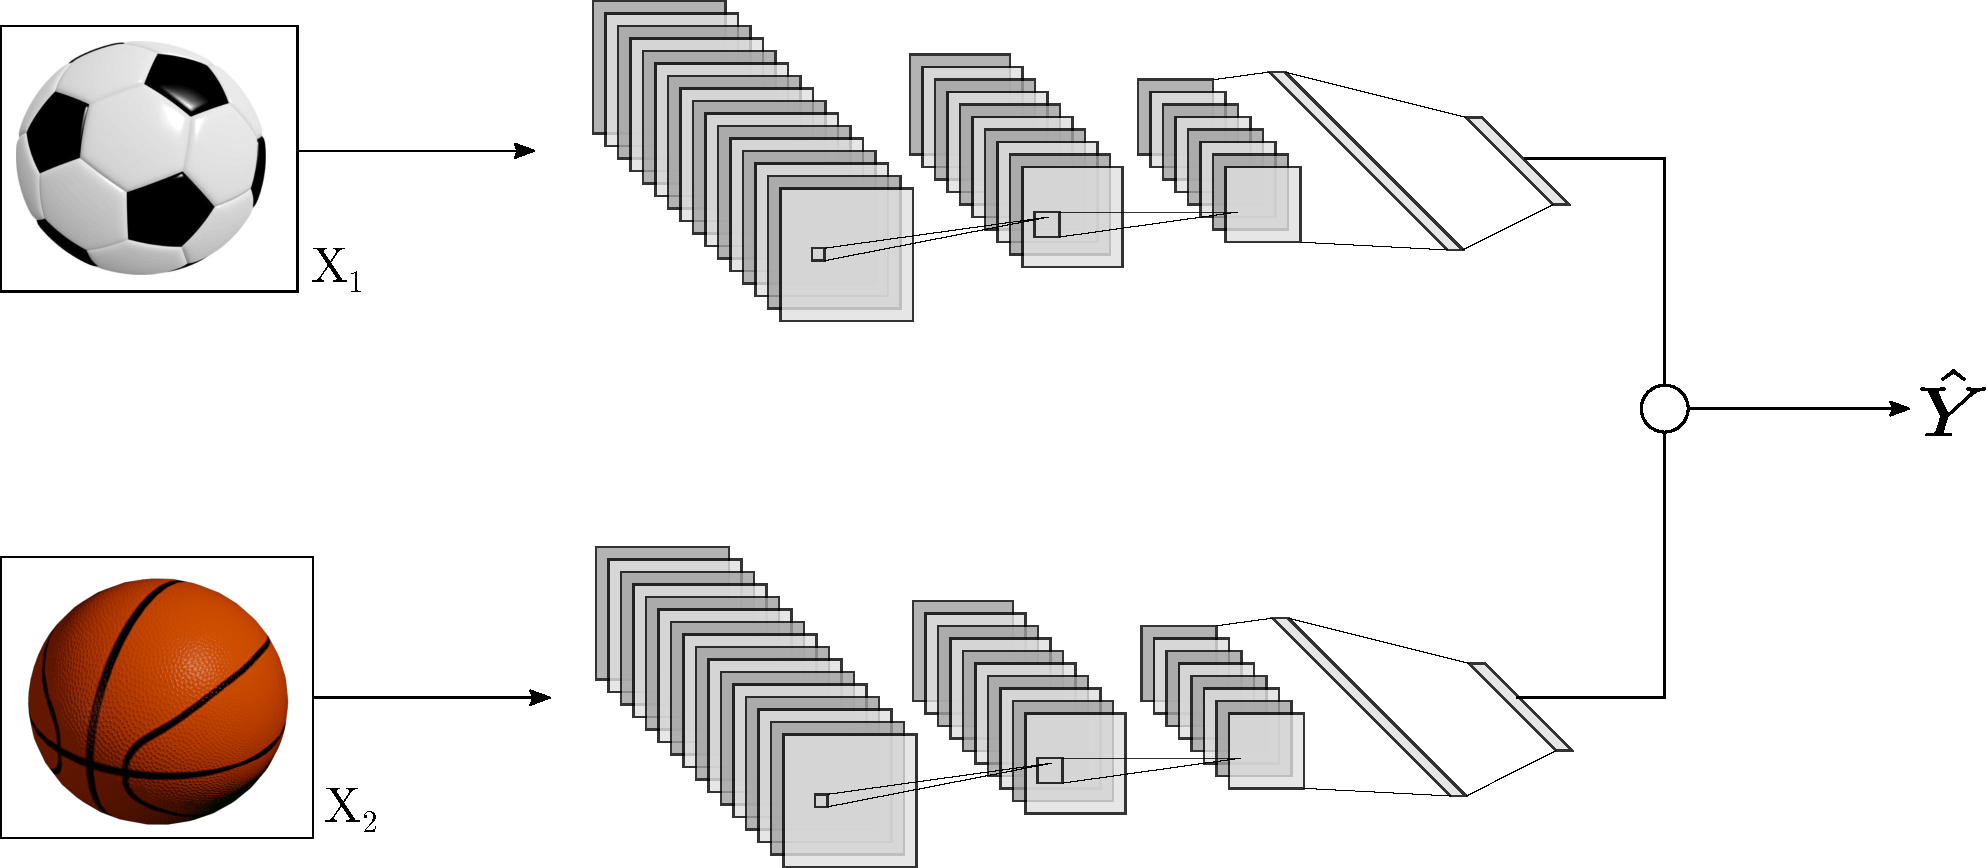
\includegraphics[width=0.8\textwidth]{img/siamese_balls}
	\caption[Siamese DNN]{Siamese Neural Networks.}
	\label{fig:siamese}
\end{figure}


\subsection{Generative Adversarial Networks (GAN)}
\label{ssec:GAN}
The Generative Adversarial Networks (GAN) were introduced by Ian Goodfellow et al. in 2014 \cite{goodfellow2014generative} with the aim to artificially generate photographs with many realistic characteristics, looking authentic to human observers. The architecture is composed of two networks: one generates candidates (generative), while the other network evaluates them (discriminative). Typically, the generative network learns to map from a latent space to a particular data distribution of interest, while the discriminative network classify the data produced by the generator between instances from the true data distribution and synthetic data. The generative network's training objective is to increase the error rate of the discriminative network (i.e., "fool" the discriminator network by producing novel synthesized instances that appear to have come from the true data distribution). The objective function of the discriminative is instead a more traditional binary classification cost function (i.e., binary cross-entropy). 

In \cite{makhzani2015adversarial}, adversarial autoencoders have been introduced with the objective of turning an autoencoder into a generative model (\figref{fig:adv_goodfellow}). In particular, the encoder portion of the network learns to convert a data distribution into a prior distribution. On the other side, the decoder learns to map a prior distribution into the data distribution, indeed becoming a generative network. The discriminator network operates between the encoder and the decoder: it takes as input data generated by the encoder or data sampled from the prior distribution and it gives as output the probability of the data of being generated by the encoder. 

\begin{figure}[h]
	\centering
	\def\svgwidth{0.5\columnwidth}
	\input{2_background/img/goodfellow_approach.pdf_tex}
	\caption[Generative Adversarial Networks]{The adversarial autoencoder approach proposed in \cite{makhzani2015adversarial}. $\tilde{\boldsymbol{y}}$ is the output of the encoder, and $\boldsymbol{y}$ represents data sampled from a prior distribution.} 
	\label{fig:adv_goodfellow}
\end{figure}


\subsection{Recurrent Neural Networks (RNN)}

The Recurrent Neural Networks (RNN)s are a particular neural architecture designed to make use of the information obtained from prior network states, therefore giving the network the capability to ``remember'' past context information. This feature is obtained by adding a set of recursive connections going from and to each hidden neuron. Due this characteristic, the output is now computed only after a batch of input frames are forwarded into the network so that the final decision will rely on the correlation between different adjacent frames. Indeed, these characteristics place the RNNs in close connection with the audio processing, due to the sequential nature of the signal, which depends of its temporal evolution.
In practice, two are the typologies which have been highly employed in addition to the ``standard'' RNNs: the network based on the Long Short Term Memory (LSTM) units and on the Gated Recurrent Unit (GRU). Both of these architectures rely on computational units which act as memory blocks, thus they are able to encapsulate mid-long term characteristics of the audio signal.
In addition to the memory blocks, the bidirectional RNNs~\cite{schuster1997bidirectional} are also common architectures.
A bidirectional RNN can access context from both temporal directions, which makes it suitable i.e. for speech recognition, where whole utterances are decoded. This is achieved by processing the input data in both directions with two separate hidden layers.
Both hidden layers are then fed to the output layer.

\subsubsection{Long Short Term Memory (LSTM)} Compared to a conventional RNN, in the LSTM RNN \cite{Hochreiter97-LST} the hidden units are replaced by so-called memory blocks.
These memory blocks can store information in the `cell variable' $\boldsymbol{c}_t$.
In this way, the network can exploit long-range temporal context.
Each memory block consists of a memory cell and three gates: the input gate, output gate, and forget gate, as depicted in \figref{fig:lstm}.

\begin{figure}[h]
	\centering
	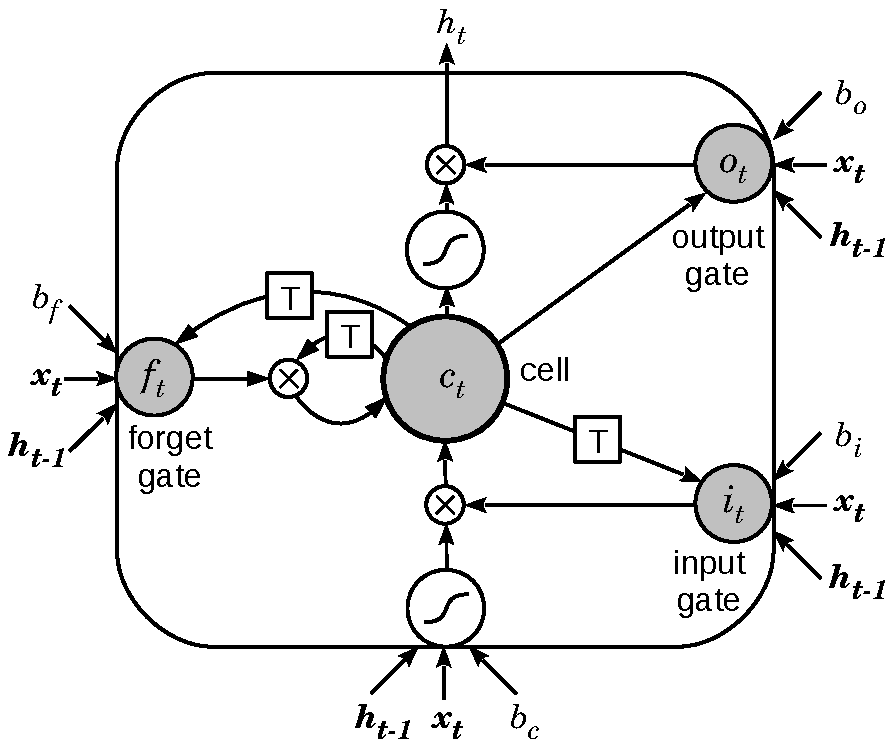
\includegraphics[width=0.5\textwidth]{img/lstm}
	\caption[LSTM]{Long Short-Term Memory block, containing a memory cell and the input, output, and forget gates}
	\label{fig:lstm}
\end{figure}

These gates control the behaviour of the memory block.
The activation vector of each gate is computed as, for example for the input gate,
\begin{equation}
\boldsymbol{i}_t = \tanh(\boldsymbol{W}_{xi}\boldsymbol{x}_t + \boldsymbol{W}_{hi}\boldsymbol{h}_{t-1} + \boldsymbol{W}_{ci}\boldsymbol{c}_{t-1} + \boldsymbol{b}_i).
\label{eq:lstmgate}
\end{equation}
The forget gate can reset the cell variable which leads to `forgetting' the stored input $\boldsymbol{c}_t$,
while the input and output gates are responsible for reading input from $\boldsymbol{x}_t$ and writing output to $\boldsymbol{h}_t$, respectively:
\begin{equation}
\boldsymbol{c}_t = \boldsymbol{f}_t \otimes \boldsymbol{c}_{t-1} + \boldsymbol{i}_t \otimes \tanh(\boldsymbol{W}_{xc}\boldsymbol{x}_t + \boldsymbol{W}_{hc}\boldsymbol{h}_{t-1} + \boldsymbol{b}_c)
\label{eq:lstmcell}
\end{equation}
\begin{equation}
\boldsymbol{h}_t = \boldsymbol{o}_t \otimes \tanh (\boldsymbol{c}_t)
\label{eq:lstmoutput}
\end{equation}
where $\otimes$ denotes element-wise multiplication and the activation function (here the $\tanh$) is also applied in an element-wise fashion.
The variables $\boldsymbol{i}_t$, $\boldsymbol{o}_t$, and $\boldsymbol{f}_t$ are the output of the input gates, output gates and forget gates, respectively, $\boldsymbol{b}_c$ is a bias term, and $\boldsymbol{W}$ is a weight matrix.
Each memory block can be regarded as a separate, independent unit.
Therefore, the activation vectors $\boldsymbol{i}_t$, $\boldsymbol{o}_t$, $\boldsymbol{f}_t$, and $\boldsymbol{c}_t$ are all of the same size as $\boldsymbol{h}_t$, i.\,e., the number of memory blocks in the hidden layer.
Furthermore, the weight matrices from the cells to the gates are diagonal, which means that each gate depends only on the cell within the same memory block.


\subsubsection{Gated recurrent units (GRU)}
\label{sssec:GRU}
Gated recurrent units (GRUs) are a gating mechanism in recurrent neural networks, introduced in 2014 \cite{chung2014empirical}. Their performance on polyphonic music modeling and speech signal modeling was found to be similar to that of LSTMs. However, GRUs have been shown to exhibit better performance on smaller datasets. 
GRU layers control the information flow through a gated unit structure, which depends on the layer input, on the activation at the previous frame and on the reset gate.
For frame $t$, the total activation of GRU layer is a linear interpolation of previous activation $h_{t-1}$ and the candidate activation $h_t$ as:
\begin{equation}
\boldsymbol{h}_t  = \boldsymbol{u}_t  \cdot \boldsymbol{h}_{t-1}  + (1 - \boldsymbol{u}_t ) \cdot \boldsymbol{h}_t ,
\end{equation}
where $\boldsymbol{u}_t$ denotes the update gate. 
Candidate activation $\boldsymbol{h}_t$ is a function of $ \boldsymbol{h}_{t-1}$, the GRU layer’s input  $\boldsymbol{x}_{t}$ and the reset gate ${r}_{t}$. $tanh$ and $hard sigmoid$ activation functions are used for update and reset gates, respectively.
GRU's activation is mainly controlled by reset gate when the GRU layer’s input $\boldsymbol{x}_{t}$ is significantly different than in previous frames. When reset gate is closed $r_{t} = 0$, the candidate activation does not include any contribution from $\boldsymbol{h}_{t-1}$. 
Fast response to the changes in the input and the previous activation information is fundamental for high performance in the proposed algorithm, where the task is to detect a small chunk of consecutive time frames where the target event is present. 

\begin{figure}[h]
	\centering
	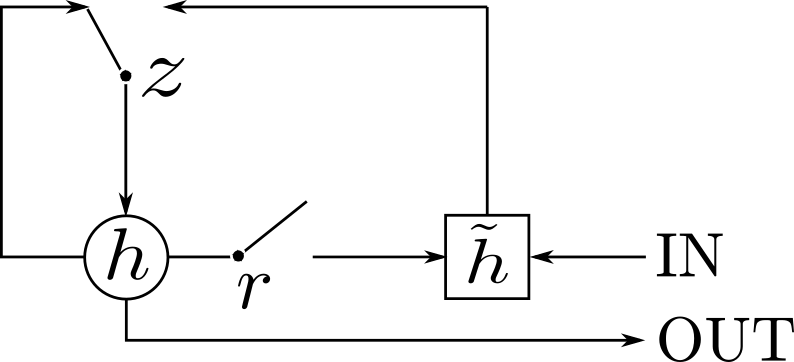
\includegraphics[width=0.6\textwidth]{img/GRU.png}
	\caption[GRU]{The Gated Recurrent Unit, containing the input, output, and forget gates}
	\label{fig:GRU}
\end{figure}


\subsection{Capsule Neural Networks (CapsNet)}

The CapsNet architecture relies on the CNN architecture and includes its computational units in the first layers of the network as invariant features extractor from the input hereafter referred as $\mathbf{X}$.
Following Hinton's preliminary works \cite{hinton2011transforming}, in the CapsNet presented in \cite{sabour2017dynamic} two layers are divided into many small groups of neurons called \textit{capsules}. In those layers, the scalar-output feature detectors of CNNs are replaced with vector-output capsules and the dynamic routing, or \textit{routing-by-agreement} algorithm is used in place of max-pooling, in order to replicate learned knowledge across space. 

Formally, we can rewrite \eqref{eq:conv_op} as
\begin{equation}
\label{eq:capsule1}
\mathbf{H}_{m}=
\begin{bmatrix} 
\alpha_{11}\mathbf{W}_{11}\mathbf{X}_1 + \ldots + 	\alpha_{M1}\mathbf{W}_{1M}\mathbf{X}_M   \\
\vdots  \\
\alpha_{1K} \mathbf{W}_{K1}\mathbf{X}_1 + \ldots + 	\alpha_{MK} \mathbf{W}_{KM}\mathbf{X}_M   \\
\end{bmatrix} .
\end{equation}
In \eqref{eq:capsule1}, $\left (\mathbf{W} \ast \mathbf{X} \right )$ has been partitioned into $K$ groups, or capsules, so that each row in the column vector corresponds to an output capsule (the bias term $\mathbf{b}$ has been omitted for simplicity).
Similarly, $\mathbf{X}$ has been partitioned into $M$ capsules, where $\mathbf{X}_i$ denotes an input capsule $i$, and  $\mathbf{W}$ has been partitioned into submatrices $\mathbf{W}_{ij}$ called \textit{transformation matrices}. Conceptually, a capsule incorporates a set of properties of a particular entity that is present in the input data. With this purpose, coefficients 
$\alpha_{ij}$ have been introduced. They are called \textit{coupling coefficients} and if we set all the $\alpha_{ij} = 1$, \eqref{eq:conv_op} is obtained again.

The coefficients $\alpha_{ij}$ affect the learning dynamics with the aim to represent the amount of agreement between an input capsule and an output capsule. In particular, they measure how likely capsule $i$ may activate capsule $j$, so the value of $\alpha_{ij}$ should be relatively accentuated if the properties of capsule $i$ coincide with the properties of capsule $j$ in the layer above.
The coupling coefficients are calculated by the iterative process of dynamic routing to fulfill the idea of assigning parts to wholes. 
Capsules in the higher layers should comprehend capsules in the layer below in terms of the entity they identify, while dynamic routing iteratively attempts to find these associations and supports capsules to learn features that ensure these connections.

In this work, we employ two layers composed of capsule units, and we denote them as Primary Capsules for the lower layer and Detection Capsules for the output layer throughout the rest of the paper.


\subsubsection{Dynamic Routing}
\label{ssec:routing}

After giving a qualitative description of routing, we describe the method used in \cite{sabour2017dynamic} to compute the coupling coefficients.
The activation of a capsule unit is a vector which holds the properties of the entity it represents in its direction. 
The vector's magnitude indicates instead the probability that the entity represented by the capsule is present in the current input.
To interpret the magnitude as a probability, a \textit{squashing} non-linear function is used, which is given by:
\begin{equation}
\label{eq:squashing}
\begin{split}
\mathbf{v}_j & = \frac{\| \mathbf{s}_j \|^2}{ 1 + \| \mathbf{s}_j \|^2} \frac{\mathbf{s}_j}{ \|\mathbf{s}_j \|}  \\
\end{split},
\end{equation}
where $\mathbf{v}_j$ is the vector output of capsule $j$ and $\mathbf{s}_j$ is its total input. $\mathbf{s}_j$ is a weighted sum over all the
outputs $\mathbf{u}_i$ of a capsule in the Primary Capsule layer multiplied by the coupling matrix $\mathbf{W}_{ij}$:

\begin{equation}
\label{eq:capsule2}
\mathbf{s}_j = \sum_{i}{} \alpha_{ij}\hat{\mathbf{u}}_{j|i},  ~ \hat{\mathbf{u}}_{j|i} = \mathbf{W}_{ij}\mathbf{u}_i.
\end{equation}
The routing procedure work as follows. The coefficient $\beta_{ij}$ measures the coupling between the $i$-th capsule from the Primary Capsule layer and the $j$-th capsule of the Detection Capsule layer. The $\beta_{ij}$ are initialized to zero, then they are iteratively updated by measuring the agreement between the current output $\mathbf{v}_j$ of each capsule in the layer $j$ and the prediction $\hat{\mathbf{u}}_{j|i}$ produced by the capsule $i$ in the layer below. 
The agreement is computed as the scalar product 
\begin{equation}
c_{ij} = \mathbf{v}_j \cdot \hat{\mathbf{u}}_{j|i},
\end{equation}
between the aforementioned capsule outputs. It is a measure of how similar the directions (i.e., the proprieties of the entity they represent) of capsules $i$ and $j$ are. 
The $\beta_{ij}$ coefficients are treated as if they were log likelihoods, thus the agreement value is added to the value owned at previous routing step:
\begin{equation}
\label{eq:routing_update}
\beta_{ij} (r + 1) =  \beta_{ij} (r) + c_{ij} (r)  =   \beta_{ij} (r) + \mathbf{v}_j \cdot \hat{\mathbf{u}}_{j|i} (r), 
\end{equation}
where $r$ represents the routing iteration. In this way the new values for all the coupling
coefficients linking capsule $i$ to higher level capsules are computed.
To ensure that the coupling coefficients $\alpha_{ij}$ represent log prior probabilities, the softmax function to $\beta_{ij}$ is computed at the start of each new routing iteration. Formally:
\begin{equation}
\alpha_{ij} = \frac{\exp(\beta_{ij})}{\sum_{k}\exp(\beta_{ik})},
\end{equation}
so $ \begin{matrix}\sum_{j}^{} \alpha_{ij} = 1 \end{matrix}$.
Thus, $\alpha_{ij}$ can be seen as the probability that the entity represented by capsule Primary Capsule $i$ is a part of the entity represented by the Detection Capsule $j$ as opposed to any other capsule in the layer above.

%\begin{figure}[tb]
%	\centering
%	\includegraphics[width=\columnwidth]{imgs/alg.jpg}
%	\label{fig:routing}
%	\caption{The routing algorithm. Source taken from \cite{sabour2017dynamic}.}
%\end{figure}

\subsubsection{Margin loss function}
The length of the vector $\mathbf{v}_j$ is used to represent the probability that the entity represented by the capsule $j$
exists.
The CapsNet have to be trained to produce long instantiation vector at the corresponding $k_{th}$ capsule if the event that it represents is present in the input audio sequence.
A separate margin loss is defined for each target class $k$ as:
\begin{equation}
\begin{split}
L_k = T_k \max(0, m^+ - & \left \|\mathbf{v}_j \right \|)^2 + \\
&\lambda(1 - T_k)\max(0, \left \|\mathbf{v}_j \right \| - m^-)^2
\end{split}
\end{equation}
where $T_k = 1$ if an event of class $k$ is present, while $\lambda$ is a down-weighting factor of the loss for absent sound event classes classes. 
$m^+$, $ m^-$ and $\lambda$ are respectively set equal to 0.9, 0.1 and 0.5 as suggested in \cite{sabour2017dynamic}.
The total loss is simply the sum of the losses of all the Detection Capsules.



\section{Optimization Algorithms}

\begin{figure}[h]
	\center
	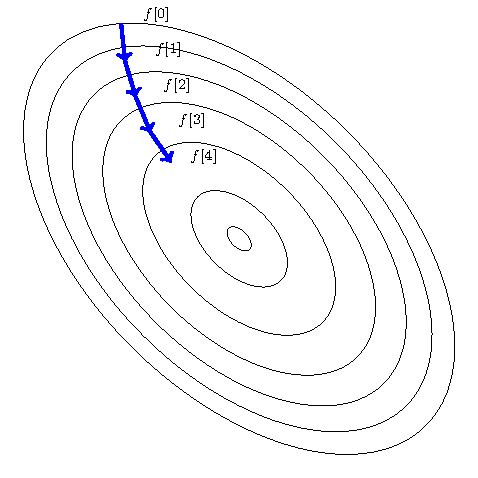
\includegraphics[width=0.550\textwidth]{img/gradient_descent}
	\caption[Example of Gradient Descent]{An example of the application of gradient descent to search for minimum of a function in a figurative 2-D plane. The process is iterated four times, while the small central ellipse corresponds to the minimum of the function.}
	\label{fig:gradient_descent}
\end{figure}

Most deep learning training algorithms involve optimization of some sort.
The most widely used is the gradient based optimization, which belongs to the first order type.
\textit{Optimization} is the task of either minimizing some function $f(x)$ by altering $x$:
$f(x)$ is called \textit{objective function}, but in the case when it has to be minimized, it is also call the \textit{cost function}, \textit{loss function}, or \textit{error function}.
The aim of the optimization is reached doing small change $\epsilon$ in the input $x$, to obtain the corresponding change in the output $f(x)$:
\begin{equation}
f(x+\epsilon) \approx f(x)+\epsilon\,f'(x).
\end{equation}
This formulation is based on the calculation of the derivative $f'(x)$.
The \textit{gradient descent} is the technique based on the reduction of $f(x)$ by moving $x$ in small steps with the opposite sign of the derivative.
The aim is to find the minimum of the cost function: when $f'(x)=0$, the derivative provides no information about which direction to move, therefore this point is defined as stationary points.
A local minimum is a point where $f(x)$ is lower than at all neighbouring and it is no longer possible to decrease $f(x)$ by making infinitesimal steps.
The absolute lowest value of $f(x)$ is a \textit{global minimum}.
For the concept of minimization to make sense, there must still be only one (scalar) output.
For functions that have multiple inputs $f: \R^n \rightarrow \R$, the concept of \textit{partial derivatives} is introduced.
The gradient $\nabla_{\mathbf{x}}f(\mathbf{x})$ is the vector containing all the partial derivatives.


The method of \textit{steepest descent} or \textit{gradient descent} states that decrease $f$ by moving in the direction of the negative gradient.
\begin{equation}
\textbf{x'} = \textbf{x} - \epsilon\,\nabla_{\mathbf{x}}f(\mathbf{x}),
\end{equation}
where $\epsilon$ is the \textit{learning rate}, a positive scalar determining the size of the step.
Large training sets are necessary for good generalization, but large training sets are also more computationally expensive.
The cost function decomposes as a sum over training example of per-example loss function:
i.e., the negative conditional log-likelihood of the training data is defined as:
\begin{equation}
J(\mathbf{\theta}) = \mathbb{E}(L(\textbf{x}, y, \mathbf{\theta})) = \frac{1}{m} \sum\limits_{i=1}^{m} L(\textbf{x}^{(i)}, y^{(i)}, \mathbf{\theta}),
\end{equation}
where $L$ is the per-example loss $L(\textbf{x}, y, \mathbf{\theta}) = - \log p(y|\textbf{x};\mathbf{\theta})$.
The gradient descent requires computing:
\begin{equation}
\nabla_{\theta} J(\mathbf{\theta}) = \frac{1}{m} \sum\limits_{i=1}^{m} \nabla_{\theta} L(\textbf{x}^{(i)}, y^{(i)}, \mathbf{\theta}).
\end{equation}
The computational cost of this operation is proportional to the number of example $m$, therefore as the training set size grows the time to take a single gradient step becomes prohibitively long.


\subsection{Stochastic Gradient Descent (SGD)}

\textit{Stochastic gradient descent} (SGD) is an extension of the gradient descent algorithm: the insight is that the gradient is an expectation estimated using a small set of samples.
On each step of the algorithm, a sample of example $\mathbb{B} = \{ \textbf{x}^{(1)}, \ldots, \textbf{x}^{(m')}\}$, called \textit{minibatch}, is drawn uniformly from the training set.
The minibatch size $m'$ is typically chosen to be a relatively small number of examples.
The estimate of the gradient is:
$\textbf{g} = \frac{1}{m'} \nabla_{\theta} \sum\limits_{i=1}^{m'} L(\textbf{x}^{(i)}, y^{(i)}, \mathbf{\theta})$
using examples from the minibatch $\mathbb{B}$.
The SGD algorithm then follows the estimated gradient downhill:
\begin{equation}
\theta \leftarrow \theta - \epsilon\,\textbf{g}
\end{equation}
where $\epsilon$ is the learning rate.


\section{Generalization Techniques}

In order to obtain more robust models, different techniques have been proposed to \textit{regularize} the weight update during the neural networks training. They have the aim to improve the generalization proprieties of the model, i.e., the ability to perform on newly unseen data as well as (in a reasonable manner) on the training set. A brief description of the most common techniques is given in the following paragraphs.

\subsection{Dropout}

Dropout \cite{srivastava2014dropout} is a regularization technique for reducing overfitting in neural networks by preventing complex co-adaptations on training data. It is a very efficient way of performing model averaging with neural networks. The term ``dropout'' refers to the operation of randomly exclude units during the training of a neural network.

Practically, during a training iteration, a percentage (drop-rate) of units for each layer where the the dropout is employed are not updated. They are selected randomly at each new step, therefore it is like we were training a network with a different layout. This allows to prevent overfitting on the training data, making  the single units more robust to the conditions changing.
 
\subsection{Batch Normalization}
Batch Normalization \cite{ioffe2015batch} is a technique which consists to add a normalization “layer” between each layers, in order to reduce the problem of internal covariate shift. In the case that the input distribution of a learning system, such as a neural network, changes, one speaks of a so-called covariate shift. If this change happens on the input of internal nodes of (deep) neural networks, it is called an internal covariate shift

An important thing to note is that normalization has to be done separately for each dimension (input neuron), over the ‘mini-batches’, and not altogether with all dimensions. Hence the name ‘batch’ normalization.
Due to this normalization “layers” between each fully connected layers, the range of input distribution of each layer stays the same, no matter the changes in the previous layer. 

Formally, given $\mathbf{x}$ inputs from the $k^{th}$ neuron, the \textit{Batch Normalization} is computed as follows:

\begin{equation}
	\hat{\mathbf{x}} = \frac{\mathbf{x}^k-\text{E}(\mathbf{x}^k)}{\sqrt{\text{Var}[\mathbf{x}^k]}}
\end{equation}


Normalization brings all the inputs centered around 0. This way, there is not much change in each layer input. So, layers in the network can learn from the back-propagation simultaneously, without waiting for the previous layer to learn. This fastens up the training of networks, leading to the possible usage of higher learning rates.





